\documentclass{article}

%%%%%%%%%%%%%%%%%%%%%%%%%
% Packages & Macros
%%%%%%%%%%%%%%%%%%%%%%%%%

% For including graphics
\usepackage{graphicx}

% For title page
\usepackage{datetime}
\newdateformat{monthyeardate}{\monthname[\THEMONTH] \THEYEAR}

% Needed above hyperref for \footnote to link to the right spot
\usepackage[symbol]{footmisc}

% For supporting linking
\usepackage{hyperref}
\hypersetup{colorlinks,urlcolor=blue,linkcolor=blue}

% For table colouring (in command line tables)
\usepackage{colortbl}

% For supporting subfigure captions
\usepackage{subcaption}

% For code formatting
\usepackage{xcolor}
\usepackage{listings}

%%%%%%%%%%%%%%%%%%%%%%%%%
% Tool-Specific Macros
%%%%%%%%%%%%%%%%%%%%%%%%%
\usepackage{xspace}

\newcommand{\args}[1] {\textit{#1}}
\newcommand{\cmd}[1] {\texttt{#1}}     % Use for command window commands, e.g., \cmd{svn up}
\newcommand{\block}[1] {\textsf{#1}}   % Use for Simulink block names, e.g., \cmd{Subsystem1}
\newcommand{\signal}[1] {\textsf{#1}}   % Use for Simulink block names, e.g., \cmd{Subsystem1}
\newcommand{\ring}[1] {\textsf{#1}} 	 % Use for files names and paths
\newcommand{\keyword}[1] {\texttt{#1}} % Use for keywords of programming languages, e.g., \keyword{while}
\newcommand{\file}[1] {\texttt{#1}} 	 % Use for files names and paths
\newcommand{\param}[1] {\textsf{#1}}   % Use for block parameter names, e.g., \param{BlockType}

% Matlab Products
\newcommand{\matlab}{\textsc{Matlab}\@\xspace}
\newcommand{\Matlab}{\textsc{Matlab}\@\xspace}
\newcommand{\Simulink}{Simulink\@\xspace}
\newcommand{\simulink}{Simulink\@\xspace}
\newcommand{\SDV}{Simulink Design Verifier\@\xspace}
\newcommand{\mpath}{\Matlab search path\@\xspace}

% Block Names (not BlockType)
\newcommand{\ds}{\block{Data Store}\@\xspace}
\newcommand{\DSM}{\block{Data Store Memory}\@\xspace}
\newcommand{\DSR}{\block{Data Store Read}\@\xspace}
\newcommand{\DSW}{\block{Data Store Write}\@\xspace}
\newcommand{\DSRW}{\block{Data Store Read/Write}\@\xspace}
\newcommand{\DSMRW}{\block{Data Store Memory/Read/Write}\@\xspace}

\newcommand{\goto}{\block{Goto}\@\xspace}
\newcommand{\from}{\block{From}\@\xspace}

\newcommand{\inport}{\block{Inport}\@\xspace}
\newcommand{\outport}{\block{Outport}\@\xspace}
\newcommand{\constant}{\block{Constant}\@\xspace}
\newcommand{\ground}{\block{Ground}\@\xspace}
\newcommand{\subsystem}{\block{Subsystem}\@\xspace}

\newcommand{\logic}{\block{Logical Operator}\@\xspace}
\newcommand{\relational}{\block{Relational Operator}\@\xspace}
\newcommand{\ifblk}{\block{If}\@\xspace}
\newcommand{\switch}{\block{Switch}\@\xspace}
\newcommand{\merge}{\block{Merge}\@\xspace}

\newcommand{\docblock}{\block{DocBlock}\@\xspace}

\newcommand{\simfunc}{\block{Simulink Function}\@\xspace}
\newcommand{\simfunccaller}{\block{Function Caller}\@\xspace}

\newcommand{\toworkspace}{\block{To Workspace}\@\xspace}
\newcommand{\fromworkspace}{\block{From Workspace}\@\xspace}

\newcommand{\tofile}{\block{To File}\@\xspace}
\newcommand{\fromfile}{\block{From File}\@\xspace}

\newcommand{\fromspreadsheet}{\block{From Spreadsheet}\@\xspace}

\newcommand{\modelref}{\block{Model Reference}\@\xspace}
\newcommand{\library}{\block{Library}\@\xspace}
\newcommand{\librarylink}{\block{Library Link}\@\xspace}

% Commonly used parameters
\newcommand{\AND}{\param{AND}\@\xspace}
\newcommand{\OR}{\param{OR}\@\xspace}
\newcommand{\NOT}{\param{NOT}\@\xspace}
\newcommand{\NOR}{\param{NOR}\@\xspace}
\newcommand{\NAND}{\param{NAND}\@\xspace}
\newcommand{\XOR}{\param{XOR}\@\xspace}
\newcommand{\NXOR}{\param{NXOR}\@\xspace}

% Common Abbreviations
% Example
\newcommand{\eg}{\textrm{e.g.,}\@\xspace}

% That Is To Say
\newcommand{\ie}{\textrm{i.e.,}\@\xspace}

% And So On
\newcommand{\etc}{\textrm{etc.}\@\xspace}

% And Others
\newcommand{\etal}{\textrm{et al.}\@\xspace}

% With Respect To
\newcommand{\wrt}{\textrm{w.r.t.}\@\xspace}

% Vice Versa
\newcommand{\vrsa}{\textrm{vice versa}\@\xspace}

% Symbols

\usepackage{amssymb}
\newcommand{\checkbox}{\makebox[0pt][l]{$\square$}\raisebox{.15ex}{\hspace{0.1em}$\checkmark$}}%
\newcommand{\uncheckbox}{$\square$~}%


\newcommand{\ToolName}{Model Comparison Utility\@\xspace}

\newcommand{\func}[1]{%
	\ifthenelse{\equal{#1}{1}}{\keyword{find\_node}}{}%
	\ifthenelse{\equal{#1}{2}}{\keyword{getHandle}}{}%
	\ifthenelse{\equal{#1}{3}}{\keyword{getPath}}{}%
	\ifthenelse{\equal{#1}{4}}{\keyword{plotTree}}{}%
	\ifthenelse{\equal{#1}{5}}{\keyword{summaryOfChanges}}{}%
	\ifthenelse{\equal{#1}{6}}{\keyword{getPathTree}}{}%
	\ifthenelse{\equal{#1}{7}}{\keyword{highlightNodes}}{}%
}

\lstdefinestyle{code}{
	frame=single,
  basicstyle=\ttfamily\small, 
  keywordstyle=\color{blue},
  identifierstyle=\color{black},
  stringstyle=\color{violet},
  commentstyle=\color{green!40!black},
  numberstyle=\color[rgb]{0.411, 0.411, 0.411},
	language=Matlab, 
	keepspaces=false, 
	columns=flexible, 
	breaklines=true,
	numbers=left,
	deletekeywords={line},
	morekeywords=[2]{slxmlcomp, compare, load_system, open_system},
	keywordstyle=[2]{\color{blue}},
	morekeywords=[3]{find_node, getHandle, getPath, getPathTree, plotTree, summaryOfChanges, highlightNodes},
	keywordstyle=[3]{\color{orange}},
}
\lstset{style=code}

%%%%%%%%%%%%%%%%%%%%%%%%%
% Text Macros
%%%%%%%%%%%%%%%%%%%%%%%%%

\newcommand{\EditsObj}{\keyword{xmlcomp.Edits}\@\xspace}
\newcommand{\NodeObj}{\keyword{xmlcomp.Node}\@\xspace}

%%%%%%%%%%%%%%%%%%%%%%%%%
% Document
%%%%%%%%%%%%%%%%%%%%%%%%%

\title{\ToolName}
\date{\monthyeardate\today}

\begin{document}

%%%%%%%%%%%%%%%%%%%%%%%%%%%%%%%%%%%%%%%%%%%%%%%%%%%%%%%%%%%%%%%%%%%
% Title Page
%%%%%%%%%%%%%%%%%%%%%%%%%%%%%%%%%%%%%%%%%%%%%%%%%%%%%%%%%%%%%%%%%%%
\maketitle
\vfill

\begin{figure}
	\centering
	
\includegraphics[]{../figs/McSCert_Logo.pdf} \\
	McMaster Centre for Software Certification (McSCert)
\end{figure}

\newpage

%%%%%%%%%%%%%%%%%%%%%%%%%%%%%%%%%%%%%%%%%%%%%%%%%%%%%%%%%%%%%%%%%%%
% Table of Contents
%%%%%%%%%%%%%%%%%%%%%%%%%%%%%%%%%%%%%%%%%%%%%%%%%%%%%%%%%%%%%%%%%%%

\tableofcontents
\newpage

%%%%%%%%%%%%%%%%%%%%%%%%%%%%%%%%%%%%%%%%%%%%%%%%%%%%%%%%%%%%%%%%%%%
% Introduction
%%%%%%%%%%%%%%%%%%%%%%%%%%%%%%%%%%%%%%%%%%%%%%%%%%%%%%%%%%%%%%%%%%%
\section{Introduction}
% Briefly, what is the tool?

Differencing between two models is natively supported in Simulink via the \href{https://www.mathworks.com/help/simulink/model-comparison.html}{Simulink Comparison Tool}. This tool relies on XML comparison techniques to generate a Word or HTML report displaying the changes that occur between models. Unfortunately, for large industrial models, these generated reports are not readable. As an alternative, the tool can output the comparison results to the \Matlab base workspace as an \EditsObj object that is structured as a tree. An example of this object's structure can be seen in Figure~\ref{FIG:tree}.

Unfortunately, MathWorks provides no built-in commands to be able to easily and programmatically query or parse this tree from the command line or a script. Manually doing so for industrial models is simply not possible. Moreover, extracting information from the tree requires thorough knowledge of the tree structure and the object parameters, and thus is not trivial without much effort. The \ToolName was created to facilitate such operations via a collection of commands. Some useful commands provided by this tool are:

\begin{itemize}
	\item \func{1} -- Search the comparison tree for nodes with specific block types, changes, names, \etc~(Section~\ref{SEC:findnode}).
	\item \func{2} -- Get the handle of the model element associated with the node from the comparison tree~(Section~\ref{SEC:gethandle}).
	\item \func{3} -- Get the pathname of the model element associated with the node from the comparison tree~(Section~\ref{SEC:getpath}).
  \item \func{6} -- Get the path of the tree element in the comparison tree~(Section~\ref{SEC:getpathtree}).
	\item \func{4} -- Plot the digraph of the comparison tree~(Section~\ref{SEC:plot}).
	\item \func{5} -- Print a summary report of the changes in the comparison tree to the Command Window or a \file{.txt} file~(Section~\ref{SEC:summary}).
	\item \func{7} -- Highlight model elements corresponding to comparison tree  nodes~(Section~\ref{SEC:highlight}).
\end{itemize}
Many other commands are included and are free to be used, but are not listed here. Please explore the source files for this utility to see all the of the various functions.

\subsection{About the Comparison Tree}

This section gives a brief overview of how a comparison tree is structured and explains some of the unintuitive aspects of the tree. A graphical representation of a comparison tree is shown in Figure~\ref{FIG:tree}. Note that there are slight differences to this tree between some \Simulink versions (\eg between R2016b, R2017b, and R2019a). 

In general, there are two kinds of objects that comprise the tree: \EditsObj and \NodeObj. The root node of a comparison tree is an \EditsObj object. It is shown in black in Figure~\ref{FIG:tree}. This object contains information about the comparison, including file names of the files being compared, filters applied during comparison, and most importantly, the hierarchical nodes that differ between the two models.  The \EditsObj properties are described in Figure~\ref{FIG:ObjectTable}. The \param{LeftRoot} and \param{RightRoot} link to the \NodeObj objects that make up each sub-tree representing each model.

\begin{figure}[!htb]
  \centering
	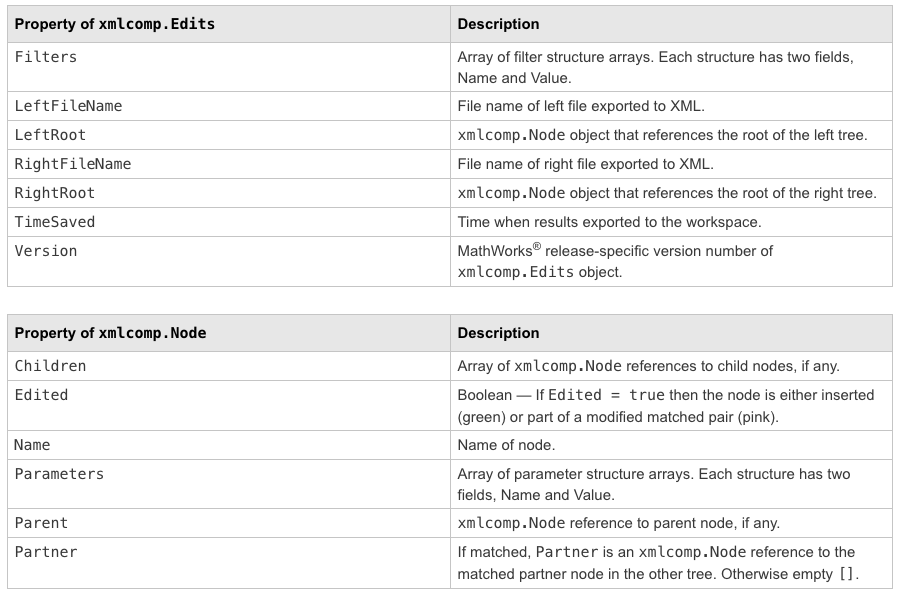
\includegraphics[width=\textwidth,]{../figs/ObjectTable}
	\caption{Properties of the comparison objects~\cite{CompareXML}.}
	\label{FIG:ObjectTable}
\end{figure}

Each element that is an \NodeObj usually represents a block, line, annotation, port, mask, or block diagram from the \Simulink model that has been changed. \Simulink model elements which have \emph{not} been changed are not included in the tree, unless they are a componentization block, such as a \subsystem, that is needed to preserve the hierarchy (\eg \block{Subsystem1} and \block{Subsystem2} in Figure~\ref{FIG:tree}. It is important to remember that the tree is only representative of the parts of the model that have changed, and unchanged parts of the model may not be represented by the tree.

An \NodeObj object's properties are described in Figure~\ref{FIG:ObjectTable}. Note that the \param{Edited} field is only set to \textit{true} when the node itself is different in the tree hierarchy (deleted, added, moved). It is not set when a node property (block parameter) is changed. The \ToolName does not rely on this field as an accurate indicator of change in the model. To determine the types of changes that occur, the \ToolName takes into account changes to the node's \param{Name}, \param{Partner}, \param{Parent}, and \param{Parameters}. Moreover, the placement in the tree is important for understanding how the element has changed, as summarized in Table~\ref{TBL:Placement}.

\begin{table}[htb] 
\centering
\begin{tabular}{lp{26em}}
\hline 
Change Type & \NodeObj Placement in the Comparison Tree\\ \hline \hline
Added       & Node exists in the right sub-tree, but not the left \\ \hline
Deleted     & Node exists in the left sub-tree, but not the right \\ \hline
Modified    & Node exists in the left and right sub-trees, and it is partnered \\ \hline
Renamed     & Node exists in the left and right sub-trees, and it is not partnered \\ \hline                                                                       
\end{tabular}
\caption{Effect of placement on an \NodeObj}
\label{TBL:Placement}
\end{table}

It is important to look at the whole tree to understand the changes. By only looking at the left sub-tree, a node that exists in the left sub-tree can be either deleted or renamed (but definitely not added or modified). By only looking at the right-subtree, a node that exists in the right-subtree can be added or modified (but definitely not deleted). Even after determining the placement of the node, it is important to check its other properties (and that of its partner) to further understand what type of change it has experienced. The \ToolName performs all of these checks automatically, so the user does not have to.

% Is there more information?
\subsection{More Information}
For more information about model comparison with \Matlab/\Simulink, please see the MathWorks documentation: \newline
\url{https://www.mathworks.com/help/simulink/model-comparison.html}

\pagebreak	
%%%%%%%%%%%%%%%%%%%%%%%%%%%%%%%%%%%%%%%%%%%%%%%%%%%%%%%%%%%%%%%%%%%
% How to Use the Tool
%%%%%%%%%%%%%%%%%%%%%%%%%%%%%%%%%%%%%%%%%%%%%%%%%%%%%%%%%%%%%%%%%%%
\section{How to Use the Tool}
This section describes what must be done to setup the tool, as well as how to use the tool.

%---------------------------------------
% What needs to be done before the tool can be used? 
% What needs to be done to a model in order for it to work on said model?
%---------------------------------------
\subsection{Prerequisites and Installation}

\begin{enumerate}
  \item Use \Matlab/\Simulink R2016b or newer.
		\begin{itemize}
			\item Note: R2016b has many bugs in the model comparison algorithm. For best results, please use R2019a+.
		\end{itemize}
	\item To install the tool, use one of the following approaches:
	\begin{enumerate}
		\item \textbf{Download the \file{.zip} from GitHub}
		\begin{enumerate} 
			\item Unzip the contents into your desired location. 
			\item Add the unzipped folder and subfolders to your \mpath. 
			\item Download the \href{https://github.com/McSCert/Simulink-Utility}{Simulink-Utility} in the same manner. Add the folder and subfolders to your \mpath also. This is a dependency for the tool to work correctly.
		\end{enumerate}
		\item \textbf{Use the Git command line}
		\begin{enumerate}
			\item Use the following command to download the tool and any necessary submodules. 
			\begin{verbatim}
			git clone --recursive https://github.com/McSCert/Model-Comparison-Utility
			\end{verbatim}
			\item Add the folder and subfolders to your \mpath. 
		\end{enumerate}
		\item \textbf{If you already have the files}
		\begin{enumerate}
			\item Add the tool folder and subfolders to your \mpath. 
		\end{enumerate}
	\end{enumerate}
	\item Run \href{https://www.mathworks.com/help/simulink/ug/registering-customizations.html}{sl\_refresh\_customizations} to refresh the Context Menu. 
	\item Ensure your model is open and unlocked.
\end{enumerate}

\paragraph{Troubleshooting:} If running the command ``\cmd{which find\_node}'' indicates that the script is not found, then the tool needs to be added to the \mpath. For information on adding files to the \mpath, please see the \href{https://www.mathworks.com/help/matlab/matlab_env/add-remove-or-reorder-folders-on-the-search-path.html}{MathWorks documentation}.
%---------------------------------------
% How/when do you access the tool?
%---------------------------------------
\subsection{Getting Started}

The utility commands are used via the \Matlab Command Window. To compare models and create a comparison tree, use the \cmd{slxmlcomp.compare} function by entering:

\begin{lstlisting}
Edits = slxmlcomp.compare(model1, model2)
\end{lstlisting}

\noindent where \cmd{model1} is the model before changes, and \cmd{model2} is the model after changes. Two example models, \file{demo\_before.mdl} and \file{demo\_after.mdl}, are provided.

\begin{lstlisting}
Edits = slxmlcomp.compare('demo_before', 'demo_after')
\end{lstlisting}

The \EditsObj object is a root node that links to two n-ary sub-trees of differences between two models. The comparison tree for the example is shown in Figure~\ref{FIG:tree}. The nodes in blue correspond to actual elements in the \Simulink models. 

%trim={<left> <lower> <right> <upper>}
\begin{figure}[!htb]
  \centering
	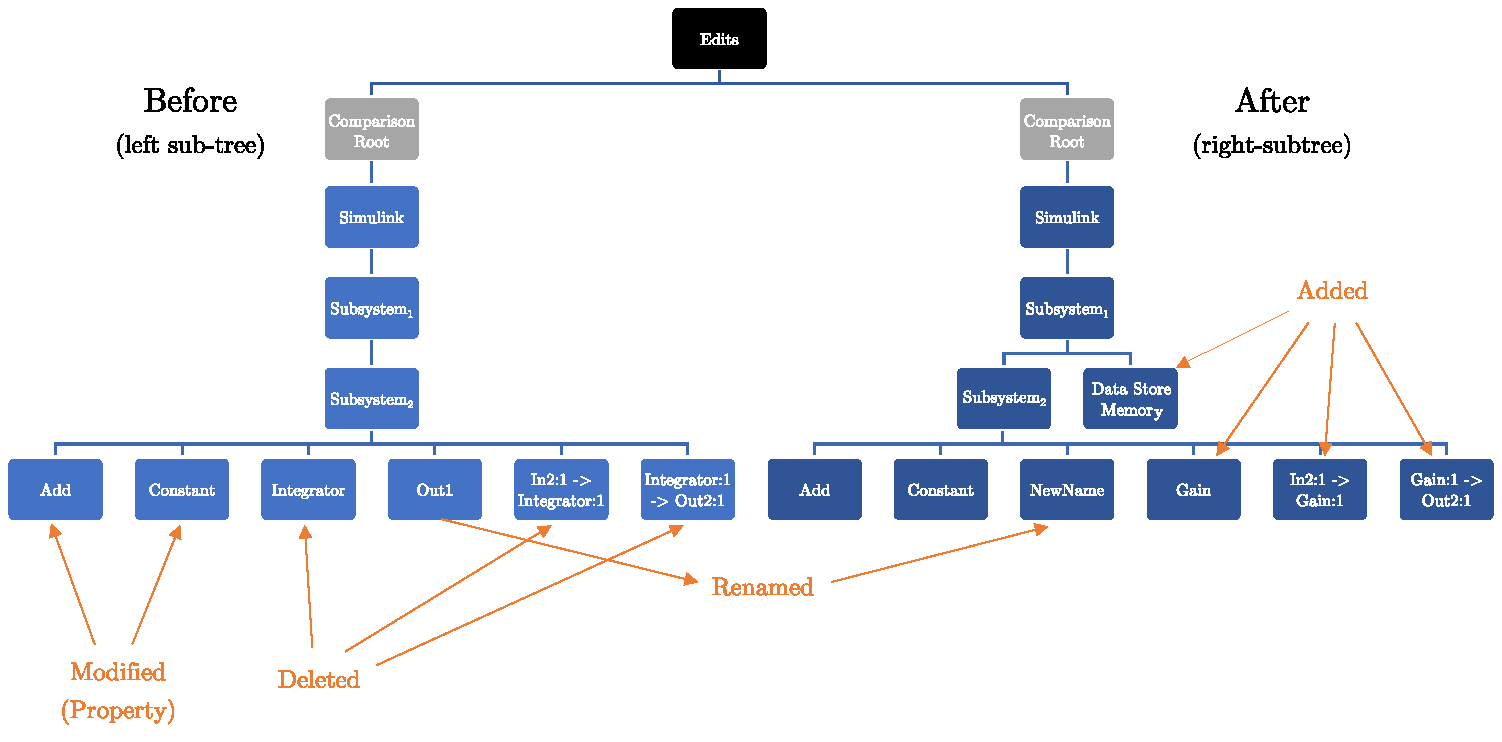
\includegraphics[width=\textheight, angle=90]{../figs/ComparisonTree}
	\caption{The \EditsObj object as created by the \Simulink Comparison Tool.}
	\label{FIG:tree}
\end{figure}

%---------------------------------------
% What are the main uses of the tool?
%---------------------------------------
\subsection{Functionality}
\label{SEC:functionality}
This section describes a few of the useful functions that are provided by the \ToolName. Full instructions on function parameters and output are given in the scripts' header comments. Feel free to explore all the scripts that are included! An example of using these functions is given in Section~\ref{SEC:example}.

\subsubsection{Finding Nodes}
\label{SEC:findnode}
A comparison tree can be comprised of numerous nodes. The \func{1} function lets you search the tree for a specific node, in a similar way that the \href{https://www.mathworks.com/help/simulink/slref/find_system.html}{\cmd{find\_system}} function searches for elements in a \Simulink model. The user can provide a list of constraints, and the function will return all nodes that fit them. It is possible to search for a node based on its change type (\eg added, deleted, modified, renamed), block type (\subsystem, \inport, \constant, \etc), block name, or node name.

\subsubsection{Getting a Node's Handle in the Model}
\label{SEC:gethandle}
One of the issues with the comparison tree is that although \NodeObj objects abstractly represent elements from the \Simulink models from which it was generated, there is no built-in way of getting a node's handle. The \func{2} function will return the node's handle, if one exists. Note that some objects do not have an associated handle in the model (\eg Mask, Comparison Root), while other objects have two handles if they exist in both sub-trees (\eg renamed block).

\subsubsection{Getting a Node's Path in the Model}
\label{SEC:getpath}
The \func{3} function returns the node's full pathname in the model.
Be aware that some model elements do not have a path (\eg lines, annotations).
Note, that if the path of the node in the tree is desired, please use the \cmd{getPathTree} function.

\subsubsection{Getting a Node's Path in the Comparison Tree}
\label{SEC:getpathtree}
The \func{6} function returns the node's full path in the comparison tree.

\subsubsection{Plotting the Comparison Tree}
\label{SEC:plot}
The \func{4} function provides a way of visually viewing the structure of a comparison tree. It plots a directed graph. Note that the full names of each node are used because unique node names are required when plotting a directed graph. The plot for the example is shown in Figure~\ref{FIG:plot}.

\begin{figure}[!htb]
  \centering
	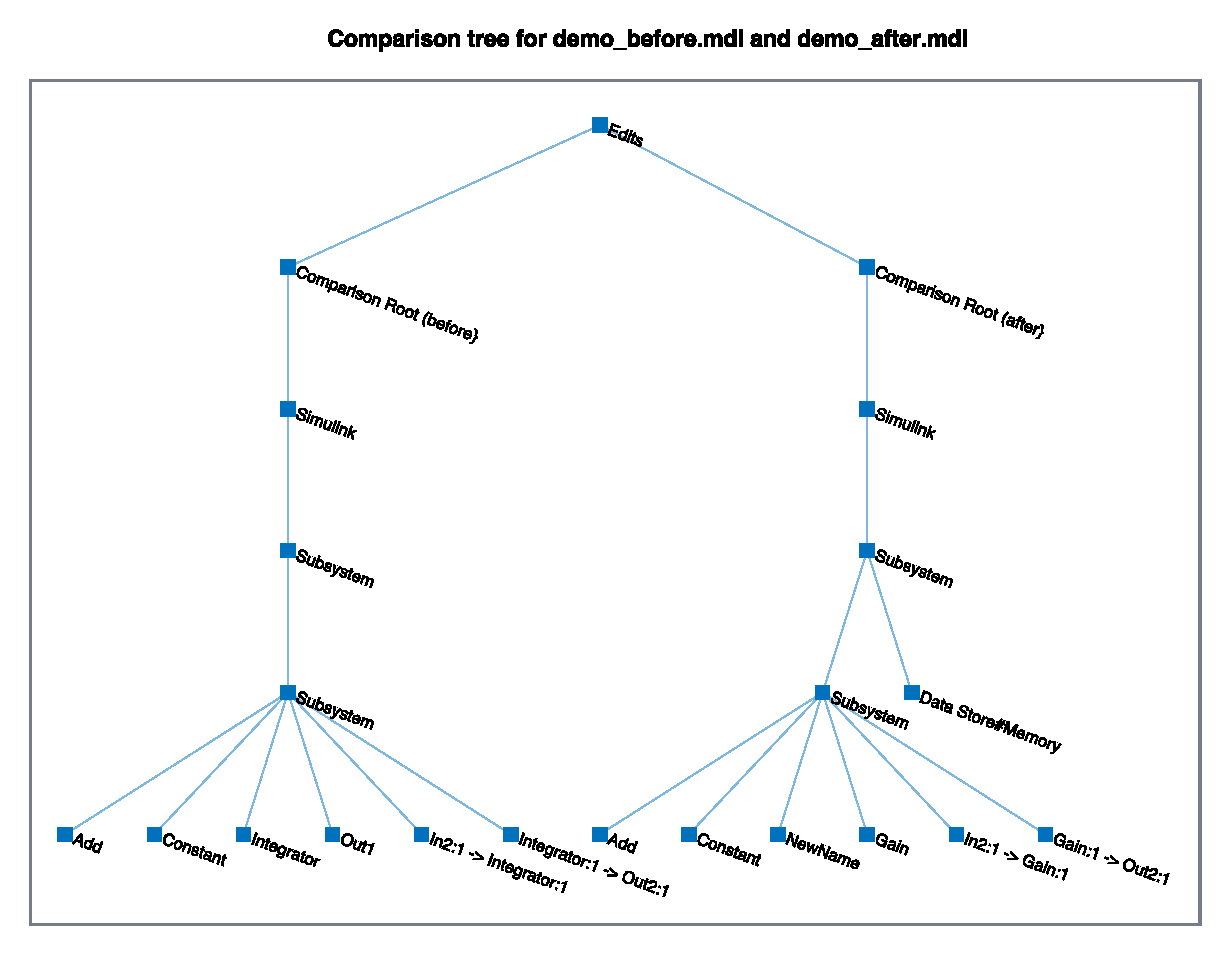
\includegraphics[width=\textwidth]{../figs/Plot}
	\caption{Plot of the comparison tree.}
	\label{FIG:plot}
\end{figure}

\subsubsection{Printing a Summary of Changes}
\label{SEC:summary}
The \func{5} function prints a text summary of the changes to a file or to the command line. Feel free to make modifications and write your own queries to include in the report.

\subsubsection{Highlight Nodes in the Model}
\label{SEC:highlight}
The \func{7} function highlights model elements corresponding to nodes. Optional arguments can be passed into the function to specify the colors and highlighting method. Please see the source code comment for more information. The highlighting can be done using the two available methods in \Simulink: using \href{https://www.mathworks.com/help/simulink/slref/hilite_system.html}{hilite\_system}, or by modifying the model element's \href{https://www.mathworks.com/help/simulink/ug/approach-modeling-programmatically.html#f4-93649}{ForegroundColor/BackgroundColor} parameters. The differences between the two approaches are elaborated on in Table~\ref{tbl:colorcomparison}. 

\begin{figure}[ht!]
\begin{center}
\begin{tabular}{p{16em} p{16em}}
\hline
 Hilite\_system & Foreground/Background \\ \hline \hline
 Highlights SubSystem blocks when they are not modified themselves & Only highlights SubSystem blocks when they are listed in the nodes argument \\ \hline
 Disappears upon model close & Can be saved in the model \\ \hline  
 Does not overwrite existing coloring &  Overwrites previous coloring \textbf{Note:} To revert to previous highlighting, do not save, and then close and reopen the model \\ \hline
 To undo, right-click in the model and select \cmd{Remove Highlighting}. & Can remove \emph{all color} (i.e. change to default black/white), by running: \cmd{highlightNodes(nodes, sys, 'fg', 'black', 'bg', 'white')} \\ \hline
 Can do highlighting on a loaded model as well as an opened model & Can do highlighting on an opened model only \\ \hline
\end{tabular}
\end{center}
\caption{The differences in highlighting methods.}
\label{tbl:colorcomparison}
\end{figure}

%%%%%%%%%%%%%%%%%%%%%%%%%%%%%%%%%%%%%%%%%%%%%%%%%%%%%%%%%%%%%%%%%%%
% Example
%%%%%%%%%%%%%%%%%%%%%%%%%%%%%%%%%%%%%%%%%%%%%%%%%%%%%%%%%%%%%%%%%%%
\section{Example}
\label{SEC:example}
Two models are provided in the \file{example} folder for demonstration purposes. They are shown in Figure~\ref{FIG:demo}. These models have several differences as a result of the following changes:

\begin{itemize}
\item 3 deleted elements:
	\begin{itemize}
		\item \block{Integrator} block was deleted (and replaced by \block{Gain} block).
		\item The two lines going into/out of \block{Integrator} are implicitly considered deleted when \block{Integrator} is deleted, and then added when \block{Gain} is connected (therefore, they are also listed as added elements).

	\end{itemize}
\item 4 added elements:
	\begin{itemize}
		\item \block{Data Store Memory} block was added.
		\item \block{Gain} block was added (in replacement of the \block{Integrator} block).
		\item The two lines going into/out of \block{Integrator} are implicitly considered deleted when \block{Integrator} is deleted, and then added when \block{Gain} is connected. 
	\end{itemize}

\item 2 modifications:
	\begin{itemize}
		\item \block{Add} block's \param{List of signs} property was changed from ++ to -- --.
		\item \block{Constant} block's \param{Constant value} property was changed from 1 to 2.
	\end{itemize}
\item 1 renamed element:
	\begin{itemize}
		\item \block{Outport} block named \param{Out1} was renamed to \param{NewName}.
	\end{itemize}
\end{itemize}

\noindent
To create the comparison tree, use the commands in the Command Window:

\begin{lstlisting}
model1 = 'demo_before';
model2 = 'demo_after';
load_system(model1);
load_system(model2);
Edits = slxmlcomp.compare(model1, model2)
\end{lstlisting}

After the \EditsObj object is created, the \ToolName can be used.

\begin{figure}[!htb]
\centering
  \begin{subfigure}[t]{.48\textwidth}
  \centering
    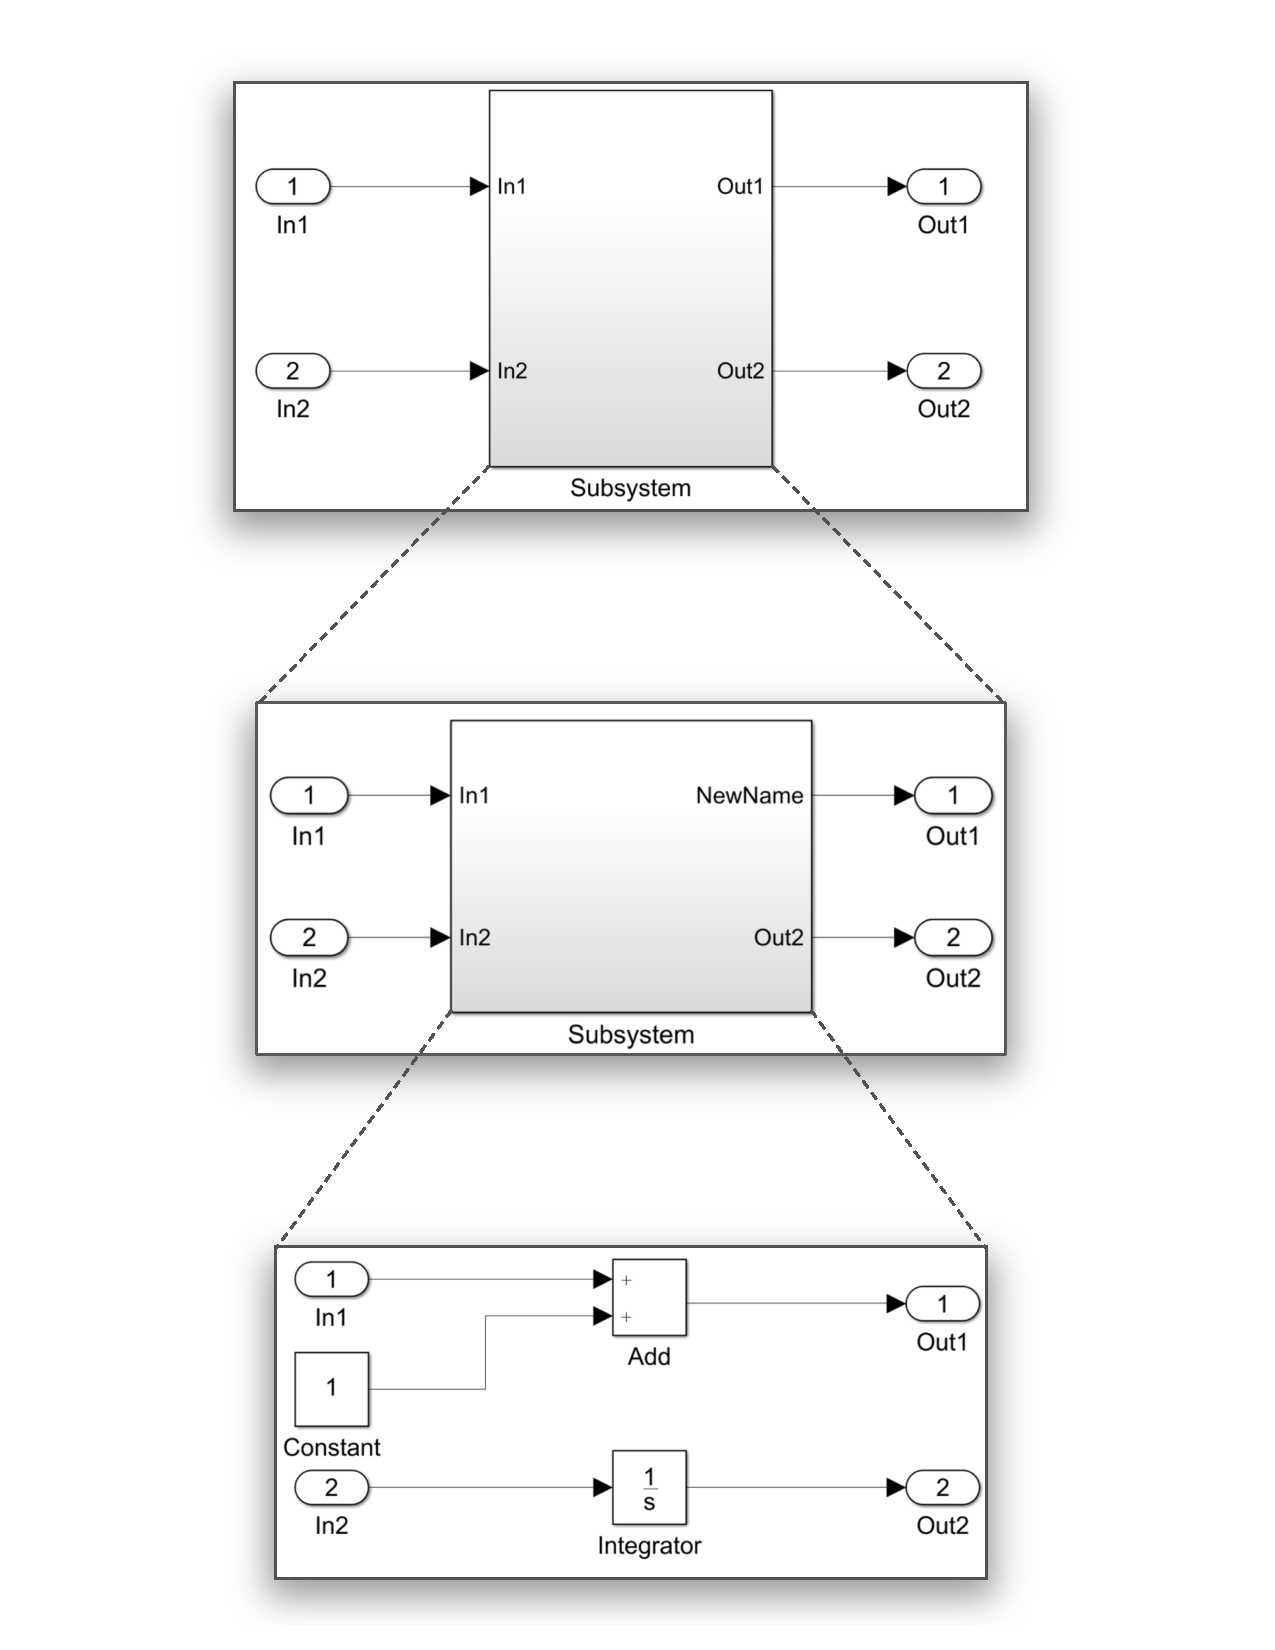
\includegraphics[width=\textwidth]{../figs/example/Before}
    \caption{Model Before Changes.}
  \end{subfigure}
  ~
  \begin{subfigure}[t]{.48\textwidth}
  \centering
    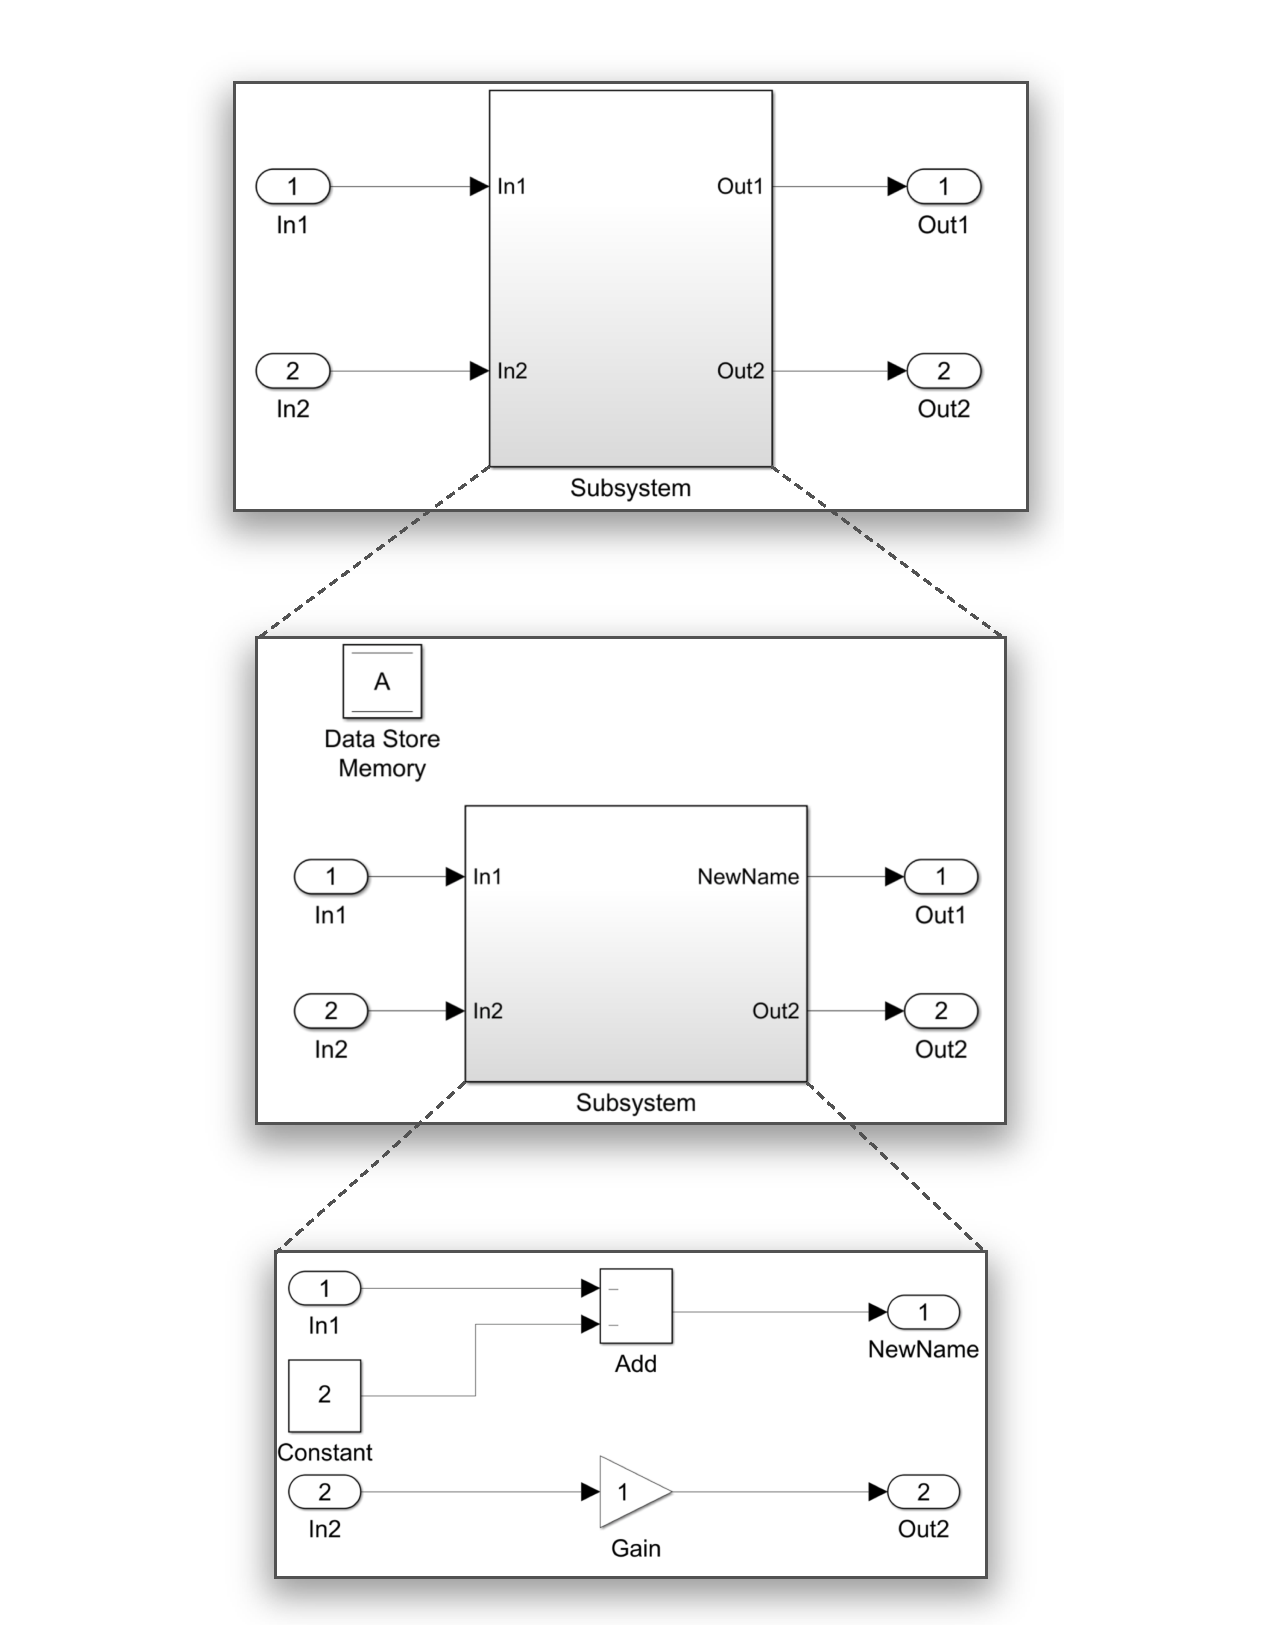
\includegraphics[width=\textwidth]{../figs/example/After}
    \caption{Model After Changes.}
  \end{subfigure}
\caption{Two Versions of a single model.}
\label{FIG:demo}
\end{figure}

\newpage
\subsection{Finding Nodes}
To find a specific set of nodes, use the \func{1} function. For example, to find only blocks that have been added, use the following command:

\begin{lstlisting}
added = find_node(Edits, 'ChangeType', 'added', 'NodeType', 'block')

added = 

  2x1 Node array with properties:

    Children
    Edited
    Name
    Parameters
    Parent
    Partner
\end{lstlisting}

\subsection{Getting a Node's Handle in the Model}
To determine the handle of one of the added nodes, use the following command. Note that because the node is added, that means that it only exists in the right sub-tree (see Table~\ref{TBL:Placement}), so we find the element in \texttt{model2}.

\begin{lstlisting}
h = getHandle(added(1), model2)

h =

   13.0004
\end{lstlisting}

\subsection{Getting a Node's Path in the Model}
To determine the path of the added node in the model, use the following command. Again, because the node is added, that means that it only exists in the right sub-tree (see Table~\ref{TBL:Placement}), so we find the element in \texttt{model2}.

\begin{lstlisting}
p = getPath(added(1), model2)

p =

    'demo_after/Subsystem/Subsystem/Gain'
\end{lstlisting}

\subsection{Getting a Node's Path in the Tree}
To determine the path of the node in the comparison tree, use the following command:

\begin{lstlisting}
pt = getPathTree(added(1))

pt =

    'Comparison Root/Simulink/Subsystem/Subsystem/Gain'
\end{lstlisting}

\subsection{Plotting the Comparison Tree}
To visualize the comparison tree, use the following command to plot it. This will display Figure~\ref{FIG:plot}.

\begin{lstlisting}
plotTree(Edits);
\end{lstlisting}

\subsection{Printing a Summary of Changes}
To print a textual report of the changes to the Command Window, use the following command. The format of the report is first the query information: $<$Query constraints$>$ -{}- TOTAL $<$\#$>$, following by the tree paths of the nodes. It is possible to print the summary to a \file{.txt} file, or omit including the paths. Please see the function's header comment for more information. Feel free to modify this report with the queries you require.

\begin{lstlisting}
>> summaryOfChanges(Edits, 1)

ChangeType, added -- TOTAL 4
   Comparison Root/Simulink/Subsystem/Subsystem/Gain
   Comparison Root/Simulink/Subsystem/Subsystem/In2:1 -> Gain:1
   Comparison Root/Simulink/Subsystem/Subsystem/Gain:1 -> Out2:1
   Comparison Root/Simulink/Subsystem/Data Store Memory
ChangeType, deleted -- TOTAL 3
   Comparison Root/Simulink/Subsystem/Subsystem/Integrator
   Comparison Root/Simulink/Subsystem/Subsystem/In2:1 -> Integrator:1
   Comparison Root/Simulink/Subsystem/Subsystem/Integrator:1 -> Out2:1
ChangeType, renamed -- TOTAL 2
   Comparison Root/Simulink/Subsystem/Subsystem/Out1
   Comparison Root/Simulink/Subsystem/Subsystem/NewName
ChangeType, modified -- TOTAL 4
   Comparison Root/Simulink/Subsystem/Subsystem/Add
   Comparison Root/Simulink/Subsystem/Subsystem/Constant
   Comparison Root/Simulink/Subsystem/Subsystem/Add
   Comparison Root/Simulink/Subsystem/Subsystem/Constant

NodeType, block, ChangeType, added -- TOTAL 2
   Comparison Root/Simulink/Subsystem/Subsystem/Gain
   Comparison Root/Simulink/Subsystem/Data Store Memory
NodeType, block, ChangeType, deleted -- TOTAL 1
   Comparison Root/Simulink/Subsystem/Subsystem/Integrator
NodeType, block, ChangeType, renamed -- TOTAL 2
   Comparison Root/Simulink/Subsystem/Subsystem/Out1
   Comparison Root/Simulink/Subsystem/Subsystem/NewName
NodeType, block, ChangeType, modified -- TOTAL 4
   Comparison Root/Simulink/Subsystem/Subsystem/Add
   Comparison Root/Simulink/Subsystem/Subsystem/Constant
   Comparison Root/Simulink/Subsystem/Subsystem/Add
   Comparison Root/Simulink/Subsystem/Subsystem/Constant

NodeType, block, ChangeType, added, BlockType, inport -- TOTAL 0
NodeType, block, ChangeType, deleted, BlockType, inport -- TOTAL 0
NodeType, block, ChangeType, renamed, BlockType, inport -- TOTAL 0
NodeType, block, ChangeType, modified, BlockType, inport -- TOTAL 0

NodeType, block, ChangeType, added, BlockType, outport -- TOTAL 0
NodeType, block, ChangeType, deleted, BlockType, outport -- TOTAL 0
NodeType, block, ChangeType, renamed, BlockType, outport -- TOTAL 2
   Comparison Root/Simulink/Subsystem/Subsystem/Out1
   Comparison Root/Simulink/Subsystem/Subsystem/NewName
NodeType, block, ChangeType, modified, BlockType, outport -- TOTAL 0

NodeType, line, ChangeType, added -- TOTAL 2
   Comparison Root/Simulink/Subsystem/Subsystem/In2:1 -> Gain:1
   Comparison Root/Simulink/Subsystem/Subsystem/Gain:1 -> Out2:1
NodeType, line, ChangeType, deleted -- TOTAL 2
   Comparison Root/Simulink/Subsystem/Subsystem/In2:1 -> Integrator:1
   Comparison Root/Simulink/Subsystem/Subsystem/Integrator:1 -> Out2:1
NodeType, line, ChangeType, renamed -- TOTAL 0
NodeType, line, ChangeType, modified -- TOTAL 0
\end{lstlisting}

\subsection{Highlighting Nodes in the Model}
To highlight nodes in the model, use the following command. Note that you must specify which model to use, and that some nodes may not exist in that model (\eg deleted nodes, added nodes).

\begin{lstlisting}
>> open_system(mdl2);
>> highlightNodes(added, mdl2);
\end{lstlisting}

\begin{thebibliography}{9}
\bibitem{CompareXML} 
The MathWorks. 
``Compare XML Files".
\\\texttt{https://www.mathworks.com/help/matlab/matlab\_env/compare-xml-files.html}
[Online; Accessed June 2020]
\end{thebibliography}

\end{document}